\documentclass{article}

\usepackage[english]{babel}

\usepackage[letterpaper,top=2cm,bottom=2cm,left=3cm,right=3cm,marginparwidth=1.75cm]{geometry}

% Useful packages
\usepackage{amsmath}
\usepackage{graphicx}
\usepackage[colorlinks=true, allcolors=blue]{hyperref}
\usepackage{listings}
\usepackage[T1]{fontenc}
\usepackage{textcomp}

\lstdefinestyle{bashStyle}{
  showstringspaces=false,
  language=bash,
  basicstyle=\small\sffamily,
  frame=tb,
  columns=fullflexible,
  linewidth=\linewidth,
  xleftmargin=0.075\linewidth,
  breaklines=true,
  literate =
    {'}{{\textquotesingle}}1
    {-}{{-}}1
}

\title{Modul 1 - Serverless Architecture}
\author{}

\begin{document}
\lstset{language=Bash,upquote=true}
\begin{figure}[h]
\centering

\includegraphics[width=0.3\textwidth]{logo.png}
\end{figure}
\centering
{\huge
Lomba Kompetensi Siswa\\
Sekolah Menengah Kejuruan\\
Tingkat Provinsi Jawa Barat\\
Tahun 2022\\
\vspace{10mm} %5mm vertical space
}
\vspace{30mm} %5mm vertical space
{\let\newpage\relax\maketitle}
\vspace{30mm} %5mm vertical space
{\LARGE Bidang Lomba Cloud Computing}

\thispagestyle{empty}
\newpage
\raggedright
\pagenumbering{arabic}

\section{Overview}
You have been tasked to deploy an API on AWS. The REST API is built using AWS serverless architecture. The data will be stored in DynamoDB. The solution requires to use a custom domain and an SSL.
\section{General Rules}
\begin{enumerate}
    \item Failure to comply with the rules will result in immediate disqualification.
    \item You have 3 hours to finish the tasks.
    \item You may not open any website unless otherwise specified in section \ref{references} and you may open the control panel of your domain provider to update the nameserver to Route 53.
    \item You may use AWS Console and AWS CLI to deploy the solutions. You may not use SAM, CloudFormation or CDK.
    \item Between and after the event, you may not access your account. Any activity on your AWS account during this period is not allowed.
    \item During the event, multiple login is not permitted.
    \item If you have any question, do not hesitate to ask.
\end{enumerate}
\section{Architecture}
\begin{figure}[h]
\centering
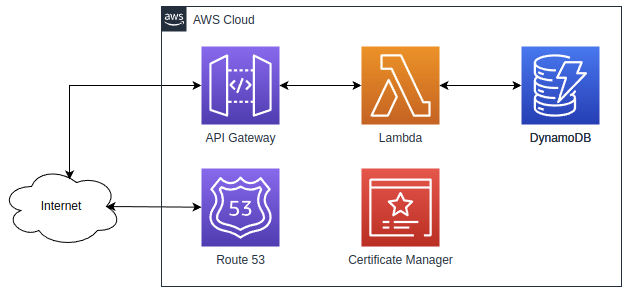
\includegraphics[width=\textwidth]{modul1_architecture.png}
\caption{\label{fig:architecture}Architecture Diagram}
\end{figure}

\section{Information}

\begin{enumerate}
  \item The repository URL for the lambda function is \href{https://github.com/kensasongko/lksccjabar2022modul1_aplikasi}{https://github.com/kensasongko/lksccjabar2022modul1\_aplikasi}
  \item This solution must be deployed in \textbf{us-east-1 (N. Virginia) region}. Deploying in another region will result in a major point reduction.
\end{enumerate}

\section{Task}
\begin{enumerate}
  \item Create a DynamoDB table with the following conditions:
  \begin{itemize}
      \item Table Name: modul1
      \item Billing Mode: Pay per request
      \item Partition Key: id
      \item Capacity Mode: On-demand
      \item Table Class: Standard
      \item Encryption Key Management: Owned by DynamoDB
      \item Tags: Key=LKS-ID, Value=MODUL1
  \end{itemize}
  \item Create and configure lambda from the repository with the following conditions:
  \begin{itemize}
      \item Add environment variables as described in the README.md from the repository.
      \item Execution time: 15 seconds
      \item Enable X-Ray tracing
      \item Tags: Key=LKS-ID, Value=MODUL1
      \item Give lambda permission to read and write DynamoDB.
  \end{itemize}
  \item Create and configure API Gateway with the following conditions:
  \begin{itemize}
      \item Protocol: REST API
      \item Endpoint Type: Edge optimized
      \item Tags: Key=LKS-ID, Value=MODUL1
  \end{itemize}
  \item Add lambda integration to the API Gateway with the following specifications:
  \begin{itemize}
      \item Resources: /todos
      \item Method: GET \& POST
      \item Set API Key Required to true on each method
  \end{itemize}
  \item Deploy the API with the following specifications:
  \begin{itemize}
      \item Stage Name: prod
      \item X-Ray tracing: enabled
  \end{itemize}
  \item Create a Usage Plan in API Gateway to limit request to the prod stage with the following specifications:
  \begin{itemize}
      \item Rate: 5 requests per second
      \item Burst: 10
      \item Quota: 1000 request per day
  \end{itemize}
  \item Create a new API Key in API Gateway.
  \item Apply the Usage Plan to the API Key.
  \item Create a certificate in ACM with the following specifications:
  \begin{itemize}
      \item Domain Name: modul1.[YOUR\_DOMAIN]
      \item Validation Method: DNS validation
      \item Tags: Key=LKS-ID, Value=MODUL1
  \end{itemize}
  \item Configure the API in the API Gateway to use custom domain with the format modul1.[YOUR\_DOMAIN]. The domain must be hosted in Route 53. 
  \item Using any REST-API-capable client (e.g., curl, Postman), ensure you can access the API using the API key you generated. Make sure the throttling works as expected.\\
  Example: 
  \begin{lstlisting}[style=bashStyle]
  $ curl -X POST \
  https://modul1.[YOUR_DOMAIN]/todos \
  -H "x-api-key: [YOUR_API_KEY]" \
  -d '{"title":"First Entry", "message":"This is the first todo entry."}'


  $ curl -X GET \
  https://modul1.[YOUR_DOMAIN]/todos \
  -H "x-api-key: [YOUR_API_KEY]"
  \end{lstlisting}
\end{enumerate}
\section{References}\label{references}
\begin{itemize}
  \item \href{https://docs.aws.amazon.com/amazondynamodb/latest/developerguide/Introduction.html}{DynamoDB documentation}
  \item \href{https://docs.aws.amazon.com/lambda/latest/dg/welcome.html}{Lambda documentation}
  \item \href{https://docs.aws.amazon.com/apigateway/latest/developerguide/welcome.html}{API Gateway documentation}
  \item \href{https://docs.aws.amazon.com/Route53/latest/DeveloperGuide/Welcome.html}{Route 53 documentation}
  \item \href{https://docs.aws.amazon.com/acm/latest/userguide/acm-overview.html}{Certificate Manager documentation}
  \item \href{https://www.postman.com/downloads/}{Postman download}
  \item \href{https://learning.postman.com/docs/getting-started/introduction/}{Postman documentation}
  \item \href{https://curl.se/download.html}{curl download}
  \item \href{https://curl.se/docs/manual.html}{curl documentation}
\end{itemize}

\section*{Good luck!}

\end{document}
